
%%%%%%%%%%%%%%%%%%%%%%%%%%%%%%%%%%%%%%%%%%%%%%%%%%%%%%%%%%%%%
\begin{frame}
\frametitle{\textbf{Project Scope}}
%------------------------------------------------------------
\begin{textblock}{110}(5,12) 
\begin{itemize}
\item \textbf{TMD fits}

  \begin{itemize}
  \item[+] single fits $\to$ Maximun Likelihood (ML)  
  \item[+] MC fits  $\to$ Nested Sampling (NS)  
  \end{itemize}

\item \textbf{Impact studies for future measurements}

  \begin{itemize}
  \item[+] Reweighting MC samples with new pseudo data sets
  \end{itemize}

\item \textbf{Data visualization}

  \begin{itemize}
  \item[+] Dedicated data vs theory visualization
  \item[+] TMD plotter
  \end{itemize}

\item \textbf{Cross section simulation}

  \begin{itemize}
  \item[+] Evaluation of cross sections 
  \item[+] Single particle MCEG
  \end{itemize}
  
\end{itemize}
\end{textblock}
%------------------------------------------------------------
\end{frame}

%%%%%%%%%%%%%%%%%%%%%%%%%%%%%%%%%%%%%%%%%%%%%%%%%%%%%%%%%%%%%
\begin{frame}
\frametitle{\textbf{Road Map}}
%------------------------------------------------------------
\begin{textblock}{100}(5,5) 
\begin{tikzpicture}%[transform canvas={scale=1.0}]
\draw[step=0.8cm,gray,very thin,opacity=0.0] (-6,-4.5) grid (6,4.5);

\node[block,fill=blue!5,text width=2cm,ultra thick] 
at (-4,3.2)(sidis) {\bf SIDIS data };

\node[block,fill=blue!5,text width=2cm,ultra thick] 
at (0,3.2)(sia) {\bf SIA data};

\node[block,fill=blue!5,text width=2cm,ultra thick] 
at (4,3.2)(pp) {\bf pp data};

\node[block,fill=yellow,text width=2.3cm,ultra thick] 
at (0,1.2)(jam) {\bf \small JAM3D source code};

\draw [orange, ->, ultra thick]  (sidis) -- (jam);
\draw [orange, ->, ultra thick]  (sia) -- (jam);
\draw [orange, ->, ultra thick]  (pp) -- (jam);


\node[block,fill=green!20,text width=2.3cm,ultra thick] 
at (-3.5,-0.5)(MC) {\bf \small TMD MC samples};

\node[block,fill=green!20,text width=2.3cm,ultra thick,minimum height=0.8cm] 
at (3.5,-0.5)(ML) {\bf \small TMD ML sample};

\draw [orange, ->, ultra thick]  (jam) -- (MC);
\draw [orange, ->, ultra thick]  (jam) -- (ML);


\node[block,fill=red!20,text width=3cm,ultra thick,minimum height=0.8cm]
at (-4,-2)(IS) {\bf \small Impact studies};

\node[block,fill=red!20,text width=3cm,ultra thick,minimum height=0.8cm]
at (-4,-3.5)(DV) {\bf \small Data/TMD visualization };

\draw [orange, ->, ultra thick]  (MC) -- (IS);
\draw [orange, ->, ultra thick]  (MC) -- (-6.0,-0.5) -- (-6,-3.5) --(DV);

\node[block,fill=red!20,text width=3cm,ultra thick,minimum height=0.8cm]
at (4,-2)(XS) {\bf \small Cross section calculator};

\node[block,fill=red!20,text width=3cm,ultra thick,minimum height=0.8cm]
at (4,-3.5)(MCEG) {\bf \small MCEG};

\draw [orange, ->, ultra thick]  (ML) -- (XS);
\draw [orange, ->, ultra thick]  (ML) -- (6.0,-0.5) -- (6,-3.5) --(MCEG);

\node[block,fill=red!20,text width=3cm,ultra thick,minimum height=0.8cm]
at (0,-2.8)(JH) {\bf \small Jupyter-Hub};


\draw [black, dashed, ultra thick]  (IS) -- (JH);
\draw [black, dashed, ultra thick]  (DV) -- (JH);

\draw [black, dashed, ultra thick]  (XS) -- (JH);
\draw [black, dashed, ultra thick]  (MCEG) -- (JH);


\draw [black, dashed, ultra thick]  (jam) -- (JH);
\draw [black, dashed, ultra thick]  (MC) -- (JH);
\draw [black, dashed, ultra thick]  (ML) -- (JH);

%\node[block,fill=red!20,text width=3cm,ultra thick,minimum height=0cm]
%at (4,-3)(la)
%{\bf \small
%\begin{minipage}{3cm}  
%\begin{itemize}
%\item Cross section calculator
%\item MCEG
%\end{itemize}
%\end{minipage}
%};




%\node[block,fill=blue!5,text width=2.5cm,ultra thick] at (4,3)(eo)
%{\bf TMD MC samples};

%\node[block,fill=blue!5,text width=2.5cm,ultra thick] at (-4,-3)(ti)
%{\bf Theory interpretation};
%\node [decision, below of=evaluate,ultra thick] at (1.5,0) (decide) 
%{\bf Does it make sense?};
%\node[block,fill=pink,text width=2.0cm,ultra thick] at (4.7,0)(paper)
%{\bf Predictions};
%
%
%\path [line,dashed, ultra thick] (decide) -- (0,-2)-- (la);
%\path [line,dashed, ultra thick] (decide) -- (0,-3)-- (ti);
%\path [line,dashed, ultra thick] (decide) -- (0,3)-- (eo);
%
%\draw [red, ->, ultra thick]  (ti) -- (eo) node 
%[text width=2.5cm,midway,above,sloped]{\bf simulation};
\end{tikzpicture}

\end{textblock}
%------------------------------------------------------------
\end{frame}

%%%%%%%%%%%%%%%%%%%%%%%%%%%%%%%%%%%%%%%%%%%%%%%%%%%%%%%%%%%%%
\begin{frame}
\frametitle{\textbf{TMD fitter }}
%------------------------------------------------------------
\begin{textblock}{110}(5,12) 
\begin{itemize}
\item \textbf{Features}
  \begin{itemize}

  \item[+] Fast evaluation of residuals $\to$ powered by dedicated 
           parallelization scripts (based on ZMQ) 

  \item[+] Parallelization can take advantage of cluster enviroments:

           \begin{itemize}
           \item[o] JLab HPCs
           \item[o] Amazon web services (AWS):  EC2, ECS  via docker
                    images
           \end{itemize}

  \item[+] Modularized framework. Easy to incorporate new observables


  \end{itemize}

\item \textbf{Methodologies}

  \begin{itemize}

  \item[+] Maximun likelhood analysis (ML)

           \begin{itemize}
           \item[o] Terminal based (``input.py'') $+$ jupyter-notebooks 
           \item[o] Also via jupyter-notebook (useful for jupyterhub
                    enviroments)
           \end{itemize}

  \item[+] MC analysis based on Nested Sampling (NS)
           \begin{itemize}
           \item[o] Terminal based (``input.py'')
           \item[o] Ideal to run on a cluster enviroment
           \end{itemize}

  \end{itemize}
 
\end{itemize}
\end{textblock}
%------------------------------------------------------------
\end{frame}


%%%%%%%%%%%%%%%%%%%%%%%%%%%%%%%%%%%%%%%%%%%%%%%%%%%%%%%%%%%%%
\begin{frame}
\frametitle{\textbf{Impact studies for future measurements}}
%------------------------------------------------------------
\begin{textblock}{110}(5,12) 
\begin{itemize}
\item \textbf{Methodology}

  \begin{itemize}
  \item[+] Simulation of new observables based on existing MC 
           samples
  \item[+] Bayesian reweighting $\to$ fastest implementation 
  \end{itemize}
  
\item \textbf{MC samples repository }

  \begin{itemize}
  \item[+] Dedicated TMD MC parameter samples generated \\ from existing 
           data
  \item[+] Access to the input files for the MC samples in case 
           new samples are need within a different setup 
          (change in parametrization, TMD theory, etc.)
  \item[+] Dedicated jupyer-notebooks templates for simulation
           and impact studies 
  \end{itemize}

\item \textbf{Jupyter-hub frontend}

  \begin{itemize}
  \item[+] No local software installation
  \item[+] Dedicated jupyer-hub server packed with JAM3D + 
           MC samples repositories 
  \item[+] Users needs to upload jupyter-notebooks from 
           from repository  
  \end{itemize}

\end{itemize}
\end{textblock}
%------------------------------------------------------------
\end{frame}


%%%%%%%%%%%%%%%%%%%%%%%%%%%%%%%%%%%%%%%%%%%%%%%%%%%%%%%%%%%%%
\begin{frame}
\frametitle{\textbf{Data visualization}}
%------------------------------------------------------------
\begin{textblock}{110}(5,12) 
\begin{itemize}
\item \textbf{Gallery of TMD studies}

  \begin{itemize}
  \item[+] Dedicated repo for jupyter-notebooks to display:
  
           \begin{itemize}
           \item[o] data vs theory
           \item[o] 2D, 3D TMDs plots (nucleon imaging)
           \end{itemize}
  \end{itemize}

\item \textbf{Jupyter-hub frontend}

  \begin{itemize}
  \item[+] No local software installation
  \item[+] Dedicated jupyer-hub server packed with JAM3D + 
           MC samples repositories 
  \item[+] Users needs to upload jupyter-notebooks from 
           from repository  
  \end{itemize}

\end{itemize}
\end{textblock}
%------------------------------------------------------------
\end{frame}


%%%%%%%%%%%%%%%%%%%%%%%%%%%%%%%%%%%%%%%%%%%%%%%%%%%%%%%%%%%%%
\begin{frame}
\frametitle{\textbf{Cross section simulation}}
%------------------------------------------------------------
\begin{textblock}{110}(5,12) 
\begin{itemize}
\item \textbf{Features}

  \begin{itemize}
  \item[+] Dedicated jupyter-notebooks for cross section evaluation
  \item[+] Dedicated jupyter-notebooks for single particle event generator
  \end{itemize}

\item \textbf{Jupyter-hub frontend}

  \begin{itemize}
  \item[+] No local software installation
  \item[+] Dedicated jupyer-hub server packed with JAM3D + 
           MC samples repositories 
  \item[+] Users needs to upload jupyter-notebooks from 
           from repository  
  \end{itemize}

\end{itemize}
\end{textblock}
%------------------------------------------------------------
\end{frame}





%
%%%%%%%%%%%%%%%%%%%%%%%%%%%%%%%%%%%%%%%%%%%%%%%%%%%%%%%%%%%%%%
%\begin{frame}
%\frametitle{\textbf{Details of  simulation (standard)}}
%%------------------------------------------------------------
%\begin{textblock}{100}(5,12) 
%\begin{tikzpicture}%[transform canvas={scale=1.0}]
%\draw[step=1cm,gray,very thin,opacity=0.0] (-6,-4) grid (6,4);
%
%\draw [red, ->, ultra thick]  (-4,-3.5)--(0.57,-3.5); 
%
%\node[block,fill=blue!5,text width=2.5cm,ultra thick] at (-4,3)(eo)
%{\bf Experimental observable};
%\node[block,fill=blue!5,text width=2.5cm,ultra thick] at (-4,-3)(ti)
%{\bf Theory interpretation};
%\node[block,fill=blue!5,text width=1.5cm,ultra thick] at (-1.2,0)(mcge)
%{\bf ``Pythia''};
%\node[block,fill=blue!5,text width=2.0cm,ultra thick] at (1.4,0)(ds)
%{\bf Detector simulation};
%\node[block,fill=blue!5,text width=2.5cm,ultra thick] at (4.5,0)(er)
%{\bf Event reconstruction};
%\node[block,fill=blue!5,text width=2.0cm,ultra thick] at (-4,0)(rw)
%{\bf Reweight};
%\node[block,fill=yellow,text width=2.5cm,ultra thick] at (2,-3)(la)
%{\bf Likelihood analysis};
%
%%\draw [orange, ->, ultra thick]  (ti) -- (-1.2,-3) -- (mcge); 
%\draw [orange, ->, ultra thick]  (mcge) -- (ds); 
%\draw [orange, ->, ultra thick]  (ds) -- (er); 
%\draw [orange, ->, ultra thick]  (er) -- (4.5,3) -- (eo); 
%
%\draw [orange, ->, ultra thick]  (ti) -- (rw); 
%\draw [orange, ->, ultra thick]  (eo) -- (rw); 
%
%\draw [red, ->, ultra thick]  (rw) -- (0,-3)--(la); 
%\end{tikzpicture}
%\end{textblock}
%%------------------------------------------------------------
%\end{frame}
%
%
%%%%%%%%%%%%%%%%%%%%%%%%%%%%%%%%%%%%%%%%%%%%%%%%%%%%%%%%%%%%%%
%\begin{frame}
%\frametitle{\textbf{Details of  simulation (ideal case)}}
%%------------------------------------------------------------
%\begin{textblock}{100}(5,12) 
%\begin{tikzpicture}%[transform canvas={scale=1.0}]
%\draw[step=1cm,gray,very thin,opacity=0.0] (-6,-4) grid (6,4);
%
%\draw [red, ->, ultra thick]  (-4,-3.5)--(0.57,-3.5); 
%
%\node[block,fill=blue!5,text width=2.5cm,ultra thick] at (-4,3)(eo)
%{\bf Experimental observable};
%\node[block,fill=blue!5,text width=2.5cm,ultra thick] at (-4,-3)(ti)
%{\bf Theory interpretation};
%\node[block,fill=blue!5,text width=1.3cm,ultra thick] at (-1.2,0)(mcge)
%{\bf MCEG};
%\node[block,fill=blue!5,text width=2.0cm,ultra thick] at (1.4,0)(ds)
%{\bf Detector simulation};
%\node[block,fill=blue!5,text width=2.5cm,ultra thick] at (4.5,0)(er)
%{\bf Event reconstruction};
%\node [decision, below of=evaluate,ultra thick] at (-4,0) (decide) 
%{\bf Does it make sense?};
%\node[block,fill=yellow,text width=2.5cm,ultra thick] at (2,-3)(la)
%{\bf Likelihood analysis};
%
%\draw [orange, ->, ultra thick]  (ti) -- (-1.2,-3) -- (mcge); 
%\draw [orange, ->, ultra thick]  (mcge) -- (ds); 
%\draw [orange, ->, ultra thick]  (ds) -- (er); 
%\draw [orange, ->, ultra thick]  (er) -- (4.5,3) -- (eo); 
%
%\draw [orange, ->, ultra thick]  (ti) -- (decide); 
%\draw [orange, ->, ultra thick]  (eo) -- (decide); 
%
%\draw [red, ->, ultra thick]  (decide) -- (0,-3)--(la); 
%\end{tikzpicture}
%\end{textblock}
%%------------------------------------------------------------
%\end{frame}
%
%
%%%%%%%%%%%%%%%%%%%%%%%%%%%%%%%%%%%%%%%%%%%%%%%%%%%%%%%%%%%%%%
%\begin{frame}
%\frametitle{\textbf{What is a likelihood analysis?}}
%%------------------------------------------------------------
%\small
%\begin{textblock}{100}(5,10)
%\begin{itemize}
%\item[+] The goal is to match experiment and theory 
%  \begin{align*} 
%  {\cal O}^{\rm Exp}(x,z,Q^2,P^{(h)}_{T},\phi_h)
%  =
%  {\cal O}^{\rm Thy}(x,z,Q^2,P^{(h)}_{T},\phi_h; 
%  {\color{red}f,d,...})
%  \end{align*} 
%\item[+]  ${\color{red}f,d}$ are theoretical functions to be fitted 
%\item[+] By construction they have the following dependence 
%  \begin{align*} 
%  f &= f(x,Q^2,k_{\perp})\\
%  d &= d(z,Q^2,p_{\perp})
%  \end{align*} 
%\item[+] In practice we need to parametrize them, e.g
%  \begin{align*} 
%  f(x,Q^2,k_{\perp})=f(x,Q^2,k_{\perp};{\color{red}\bm{a}})\\
%  d(z,Q^2,p_{\perp})=d(z,Q^2,p_{\perp};{\color{red}\bm{a}})
%  \end{align*} 
%\item[+] The individual shape parameters  $\color{red}a_i$ are not important
%      \\ \hc{$\to$ only the full function is important}
%\end{itemize}
%\end{textblock}
%%------------------------------------------------------------
%\end{frame}
%
%%%%%%%%%%%%%%%%%%%%%%%%%%%%%%%%%%%%%%%%%%%%%%%%%%%%%%%%%%%%%%
%\begin{frame}
%\frametitle{\textbf{What is a likelihood analysis?}}
%%------------------------------------------------------------
%\begin{textblock}{100}(93,7) 
%\includegraphics[width=.3\textwidth]{gallery/people/bayes}
%\end{textblock}
%%------------------------------------------------------------
%\begin{textblock}{100}(5,15) 
%\begin{itemize}
%\item \textbf{likelihood analysis using Bayesian stat.}
%\item[+]\hc{Bayes theorem}:
%  \begin{flalign*}
%  {\cal P}(f|data)&=\frac{1}{Z}{\cal L}(data|f) \pi(f) &
%  \end{flalign*}
%\item[+] The \SoulColor\hl{likelihood function} 
%  \emph{Gaussian likelihood}
%  \begin{flalign*}
%      {\cal L}(data|f) &=
%        \exp\left[-\frac{1}{2}\sum_i 
%        \left(\frac{d_i-{\rm model}_i(f)}{\delta d_i}\right)^2
%        \right]&
%  \end{flalign*}
%\item[+] The \SoulColor\hl{prior function}  to restrict 
%  unphysical regions of $f$. e.g. 
%  \begin{flalign*}
%      \pi(f)&=
%      \begin{cases} 
%      1 & {\rm condition}(f)=={\rm True} \\
%      0 & {\rm condition}(f)=={\rm False} \\
%      \end{cases}&
%  \end{flalign*}
%\end{itemize}
%\end{textblock}
%%------------------------------------------------------------
%\end{frame}
%
%
%
%%%%%%%%%%%%%%%%%%%%%%%%%%%%%%%%%%%%%%%%%%%%%%%%%%%%%%%%%%%%%%
%\begin{frame}
%\frametitle{\textbf{Likelihood analysis setup}}
%%------------------------------------------------------------
%\begin{textblock}{100}(93,7) 
%\includegraphics[width=.3\textwidth]{gallery/people/bayes}
%\end{textblock}
%%------------------------------------------------------------
%\begin{textblock}{80}(5,15) 
%\begin{itemize}
%\item In practice $f$ needs to be parametrized e.g
%\begin{flalign*}
%f(x) &= Nx^a(1-x)^b(1+c\sqrt{x}+dx+...)&\\ 
%f(x) &= Nx^a(1-x)^b{\rm NN}(x;\{w_i\})&\\ 
%f(x) &= {\rm NN}(x;\{w_i\})-{\rm NN}(1;\{w_i\})&
%\end{flalign*}
%\item The pdf for $f$ becomes
%\begin{flalign*}
%\bm{a}&=(N,a,b,c,d,...)&\\
%{\cal P}(\bm{a}|d)&=\frac{1}{Z}{\cal L}(d|\bm{a})\pi(\bm{a})&\\
%{\cal L}(d|\bm{a})&=\exp\left[-\frac{1}{2}
%                   \sum_i\left(
%                   \frac{d_i-{\rm model}_i(\bm{a})}{\delta d_i}
%                   \right)^2\right]&\\
%\pi(\bm{a})&=\prod_i \theta(a_i-a^{min}_i)\theta(a^{max}_i-a_i)& 
%\end{flalign*}
%\end{itemize}
%%------------------------------------------------------------
%\begin{textblock}{100}(57,55) 
%\begin{flalign*}
%{\cal P}(f|d)&=\frac{1}{Z}{\cal L}(d|f) \pi(f)\notag\\
%             &~~~\color{red}{\big\downarrow\notag}\\
%{\cal P}(\bm{a}|d)&=\frac{1}{Z}{\cal L}(d|\bm{a}) \pi(\bm{a})
%\end{flalign*}
%\end{textblock}
%%------------------------------------------------------------
%\begin{textblock}{1}(85,53)
%\begin{tikzpicture}
%\draw [orange,ultra thick,rounded corners](0,0) rectangle (4.2,3.2);
%\end{tikzpicture}
%\end{textblock}
%\end{textblock}
%%------------------------------------------------------------
%\end{frame}
%
%%%%%%%%%%%%%%%%%%%%%%%%%%%%%%%%%%%%%%%%%%%%%%%%%%%%%%%%%%%%%%
%\begin{frame}
%\frametitle{\textbf{Likelihood analysis setup}}
%%------------------------------------------------------------
%\begin{textblock}{100}(93,7) 
%\includegraphics[width=.3\textwidth]{gallery/people/bayes}
%\end{textblock}
%%------------------------------------------------------------
%\begin{textblock}{120}(5,15) 
%\begin{itemize}
%\item Having the pdf for $f$ we can compute
%\begin{flalign*}
%{\rm E}[\mathcal{O}] &= \int d^n a~~
%                       \mathcal{P}(\bm{a}|data)~~
%                       \mathcal{O}({\bm a}) &\\
%{\rm V}[\mathcal{O}] &= \int d^n a~~
%                        \mathcal{P}(\bm{a}|data)~~
%                        (\mathcal{O}({\bm a})-{\rm E}[\mathcal{O}])^2\notag
%\end{flalign*}
%\item $\cal O$ is any function of $\bm{a}$. e.g
%\begin{flalign*}
%{\cal O}(\bm{a})&= f(x;\bm{a}) &\\
%{\cal O}(\bm{a})&= \int_x^1 \frac{d\xi}{\xi} 
%                  C(\xi)f\left(\frac{x}{\xi};\bm{a}\right)
%\end{flalign*}
%\item How do we compute ${\rm E}[\mathcal{O}],{\rm V}[\mathcal{O}]$? 
%      \begin{itemize} 
%      \item[+] Maximum likelihood + (Hessian, Lagrange multipliers) 
%      \item[+] \hc{Monte Carlo sampling}
%      %$\color{red}{\rightarrow}$
%      \end{itemize}
%\end{itemize}
%\end{textblock}
%%------------------------------------------------------------
%\end{frame}
%
%
%%%%%%%%%%%%%%%%%%%%%%%%%%%%%%%%%%%%%%%%%%%%%%%%%%%%%%%%%%%%%%
%\begin{frame}
%\frametitle{\textbf{Nested resampling}}
%%-----------------------------------------------
%\begin{textblock}{80}(5,15) 
%\begin{itemize}
%\item \textbf{The basic idea}: compute 
%%\item [$\to$] To compute $Z$ as   
%  \begin{align} 
%  Z= \int {\cal L}({\rm data}|\bm{a}) \pi( \bm{a} )d^na
%   = \int_0^1 {\cal L}(X) dX
%   \notag
%  \end{align}
%\item[$\to$] The algorithm traverses ordered  isolikelihood contours
%      in the variable $X$ such that $X$ follows the progression 
%      $X_i=t_iX_{i-1}$
%\item[$\to$] The variable $t_i$ is estimated statistically 
%\item[$\to$] The algorithm can be optimized iteration to iteration. 
%      One can sample only in the regions where the likelihood is
%      larger $\to$ ``importance sampling''
%\item[$\to$] The nested sampling is parallelizable
%\end{itemize}
%\end{textblock}
%%------------------------------------------------------------
%\begin{textblock}{100}(90,10) 
%{\small ${\cal L}({\rm data}|\bm{a})$ in $\bm{a}$ space}\\
%\includegraphics[width=.3\textwidth]{gallery/nested-sampling/NS1}
%\end{textblock}
%%------------------------------------------------------------
%\begin{textblock}{100}(90,50) 
%{\small ${\cal L}(X)$ in $X$ space}\\
%\includegraphics[width=.3\textwidth]{gallery/nested-sampling/NS2}
%\end{textblock}
%%------------------------------------------------------------
%\end{frame}
%
%
%%%%%%%%%%%%%%%%%%%%%%%%%%%%%%%%%%%%%%%%%%%%%%%%%%%%%%%%%%%%%%
%\begin{frame}
%\frametitle{\textbf{SIDIS+Lattice analysis of nucleon tensor charge }} 
%%------------------------------------------------------------
%\begin{textblock}{150}(3,10) 
%\small
%\textbf{Lin, Melnitchouk, Prokudin, NS, Shows (arXiv:1710.09858)}
%\end{textblock}
%%------------------------------------------------------------
%\begin{textblock}{100}(1,15) 
%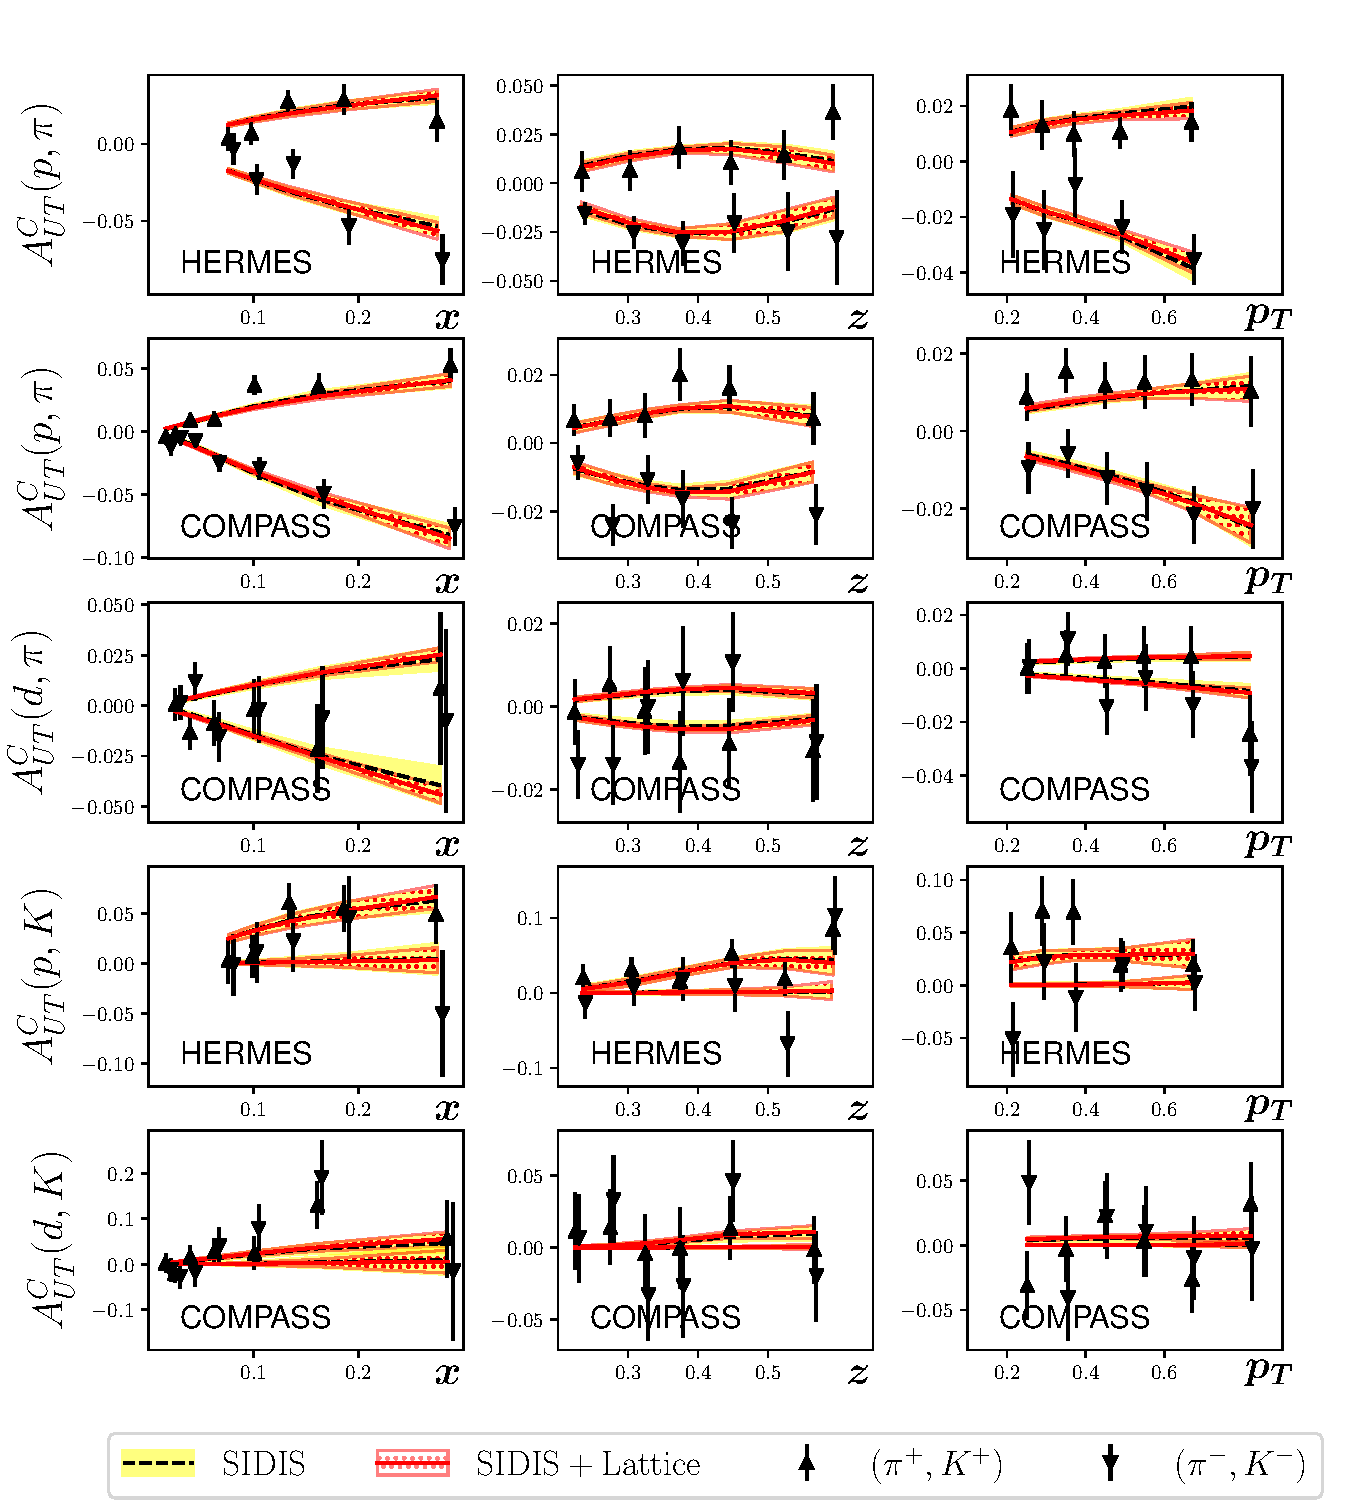
\includegraphics[width=0.6\textwidth]{gallery/tensorcharge/dvt.pdf}
%\end{textblock}
%%------------------------------------------------------------
%\begin{textblock}{100}(63,15) 
%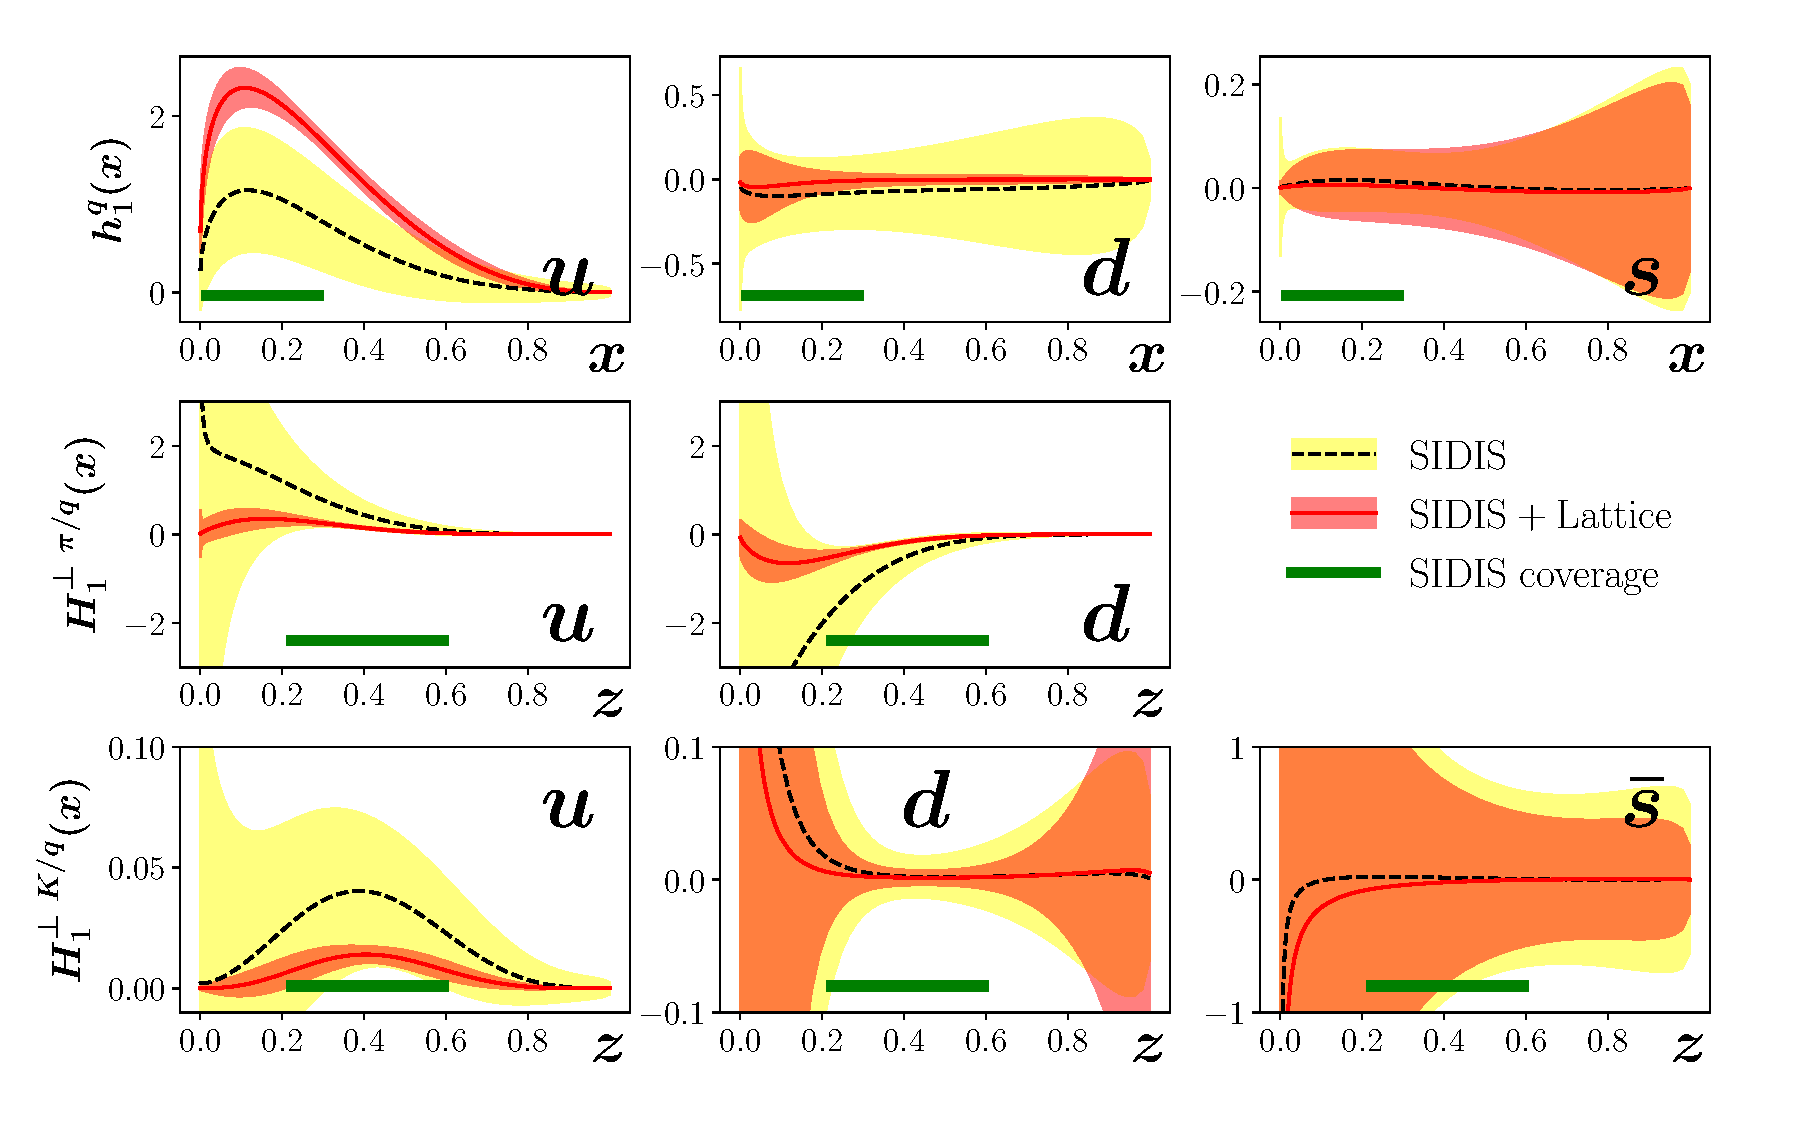
\includegraphics[width=0.6\textwidth]{gallery/tensorcharge/transversity-collins.pdf}
%\end{textblock}
%%------------------------------------------------------------
%\begin{textblock}{100}(63,38) 
%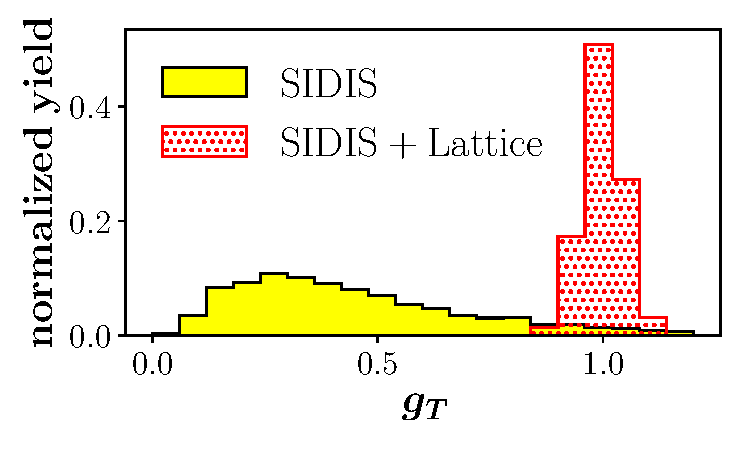
\includegraphics[width=0.6\textwidth]{gallery/tensorcharge/gT.pdf}
%\end{textblock}
%%------------------------------------------------------------
%\begin{textblock}{100}(5,60) 
%\begin{itemize}
%\item[+] Extraction of transversity and Collins FFs from SIDIS
%$A_{UT}$+Lattice $g_T$
%\item[+] In the absence of Lattice, SIDIS at present has no
%significant constraints on $g_T$ $\to$ this will change with the upcoming JLab12
%measurements
%\end{itemize}
%\end{textblock}
%%------------------------------------------------------------
%\end{frame}
%
%
%%%%%%%%%%%%%%%%%%%%%%%%%%%%%%%%%%%%%%%%%%%%%%%%%%%%%%%%%%%%%%
%\begin{frame}
%\frametitle{\textbf{Current projects}} 
%%------------------------------------------------------------
%\begin{textblock}{120}(5,10) 
%\begin{itemize}
%\item TMD physics (phenomenology): 
%  \begin{itemize}
%    \item[] \hc{ Prokudin, Tezgin, Riser, Liu, Melnitchouk, NS, ...}
%    \item[+] MC analysis on Collins function with combined SIDIS+SIA
%    \item[+] Impact studies of the SoLID experiment on Siver function 
%    \item[+] Impact studies of Belle experiment on Collins function  
%    \item[+] Impact studies of EIC on transversity (the sea distributions)
%  \end{itemize}
%\item[]
%\item TMD physics (theory)
%  \begin{itemize}
%    \item[] \hc{Rogers, Wang, Gonzalez, NS}
%    \item[+] $O(\alpha_S^2)$ corrections to fixed order $F_{UU}$ 
%    \item[+] Limits of applicability of TMD/collinear factorization 
%  \end{itemize}
%\item[]
%\item Collinear physics (phenomenology) 
%  \begin{itemize}
%    \item[] \hc{Ethier, Andres, Melnitchouk, NS, Larrieu (IT)}
%    \item[+] Universal MC analysis of PDF, $\Delta$PDF, $FF$
%             using DIS, $\Delta$DIS, SIDIS, $\Delta$SIDIS and SIA
%  \end{itemize}
%\end{itemize}
%\end{textblock}
%%------------------------------------------------------------
%\end{frame}
%
%%%%%%%%%%%%%%%%%%%%%%%%%%%%%%%%%%%%%%%%%%%%%%%%%%%%%%%%%%%%%%
%\begin{frame}
%\frametitle{\textbf{Webfitter}} 
%%------------------------------------------------------------
%\begin{textblock}{120}(5,10) 
%\begin{itemize}
%\item Goals
%  \begin{itemize}
%  \item[+] To make the pheno tools  available to everyone
%  \item[+] Eliminate unnecessary tasks of installing / compiling programs 
%  \item[+] Provide user friendly templates for impact studies 
%  \item[+] Store all the details of a given analysis  
%  \end{itemize}
%\item[]
%\item The solution $\to$ Jupyterhub
%  \begin{itemize}
%  \item[] \hc{Heffner (IT), Larrieu (IT)}
%  \item[+] It is a server for jupyter notebooks 
%  \item[+] All the codes are installed on a JLab sever 
%  \item[+] Users will be able to do any analysis on TMDs/PDFs
%           e.g. impact studies 
%  \end{itemize}
%\item[]
%\item Community driven phenomenology 
%  \begin{itemize}
%  \item[+] Template notebooks are posted on github
%          \href{https://github.com/JeffersonLab/jamfitter}{link}
%  \item[+] Users can request to upload their analysis 
%  \end{itemize}
%\end{itemize}
%\end{textblock}
%%------------------------------------------------------------
%\end{frame}

